%%%%%%%%%%%%%%%%%%%% author.tex %%%%%%%%%%%%%%%%%%%%%%%%%%%%%%%%%%%
%
% sample root file for your "contribution" to a contributed volume
%
% Use this file as a template for your own input.
%
%%%%%%%%%%%%%%%% Springer %%%%%%%%%%%%%%%%%%%%%%%%%%%%%%%%%%


% RECOMMENDED %%%%%%%%%%%%%%%%%%%%%%%%%%%%%%%%%%%%%%%%%%%%%%%%%%%
\documentclass[graybox]{svmult}

\usepackage{mathptmx}       % selects Times Roman as basic font
\usepackage{helvet}         % selects Helvetica as sans-serif font
\usepackage{courier}        % selects Courier as typewriter font
\usepackage{type1cm}        % activate if the above 3 fonts are
                            % not available on your system
%
\usepackage{makeidx}         % allows index generation
\usepackage{graphicx}        % standard LaTeX graphics tool
                             % when including figure files
\usepackage{multicol}        % used for the two-column index
\usepackage[bottom]{footmisc}% places footnotes at page bottom
\usepackage{gensymb}

% see the list of further useful packages
% in the Reference Guide

\makeindex             % used for the subject index
                       % please use the 

%%%%%%%%%%%%%%%%%%%%%%%%%%%%%%%%%%%%%%%%%%%%%%%%%%%%%%%%%%%%%%%%%%%%%%%%%%%%%%%%%%%%%%%%%

\begin{document}

\title*{Metagenomic design and sequencing}
% Use \titlerunning{Short Title} for an abbreviated version of
% your contribution title if the original one is too long
\author{William L. Trimble, Stephanie M. Greenwald, Sarah Owens, Elizabeth M. Glass, and Folker Meyer}
% Use \authorrunning{Short Title} for an abbreviated version of
\authorrunning{Trimble, et al.}
% your contribution title if the original one is too long
\institute{William L. Trimble, Stephanie M. Greenwald, and Sarah Owens  \at Institute for Genomics and Systems Biology, University of Chicago  %  \email{name@email.address} } 
   and Elizabeth M. Glass  and Folker Meyer \at Argonne National Laboratory  } %\email{name@email.address}} 

% trimble@anl.gov
% smoormann@anl.gov 
% Sarah.Owens@anl.gov
% marland@anl.gov 
% folker@anl.gov
%
%
\maketitle

% "starred" for online
\abstract*{
Metagenomics, and shotgun metagenomics in particular, is a field that has disproportionately benefited from advances in high-throughput sequencing technologies.
This chapter discusses the choice of sample number, depth, and sequencing technology, the shearing, size-selection, and multiplexing options on Illumina platforms, and outlines the steps in the bioinformatic analysis and sharing of metagenomic data.}

% Use the plain \texttt{abstract} command if the abstract is also to appear in the printed version of the book.}
\abstract{ 
Metagenomics, and shotgun metagenomics in particular, is a field that has disproportionately benefited from advances in high-throughput sequencing technologies.  
This chapter discusses the choice of sample number, depth, and sequencing technology, the shearing, size-selection, and multiplexing options on Illumina platforms, and outlines the steps in the bioinformatic analysis and sharing of metagenomic data.  }

\section{Introduction}
\label{sec:1}

The technological advances in sequencing technology in the recent decade have made determining the sequence nucleic acid polymers affordable and widespread.  While the study of variations in the genomes of model organisms including humans is a rich and fruitful area of investigation, microorganisms have vastly greater numbers and sequence diversity than macroorganisms.  Sequencing of DNA from environmental samples has become a fast-growing application of sequencing technology.

Metagenomics is the analysis of genetic material extracted from environmental samples or extracted from mixtures of organisms.  Two general approaches are available, targeted gene sequencing and random "shotgun" sequencing.    Targeted sequencing amplifies gene fragments of interest using PCR primers corresponding to conserved regions of selected genes.   Subsets of the sequence of the prokaryotic  rRNA 16S subunit, the internal transcribed spacer (ITS) in fungi, functional genes of interest to oxidation-reduction metabolism(NifH, AmoA), and conserved non-RNA phylogenetic marker genes are all suitable.  The 16S rRNA gene has proven most popular for surveying the composition of microbial communities, and as one of the genes that has been under investigation for the longest, its primers and sequences have been the most studied and have the largest number of database sequences, and protocols for high-throughput sample preparation are available.\cite{Caporaso2012Ultrahighthroughput}

Random, called "shotgun" sequencing provides unaligned samples from each organism's thousands of genes, rather than amplifying a single gene per organism or organismal type.  This increases the complexity of the sequencing data product several thousandfold, and as a result, much greater per-sample sequencing effort is required.
This higher sequencing effort has meant that environmental shotgun sequencing has been enabled disproportionately by low-cost sequencing technologies, and as a consequence the total amount of shotgun metagenomic sequence data has been rising rapidly.   The Sequence Read Archive has (as of May 2015) 34 Terabases of sequence data tagged as metagenomic in origin; IMG/M and MG-RAST claim to have 4.5  and 76 $\times 10^{12}$~bp respectively. 
Most metagenomic shotgun datasets at present have between a gigabase and a few-tens-of-gigabases sequencing effort.  
Sequencing single samples to depths of a hundred gigabases or greater have been uncommon but not unheard of.

\section{Design}

Generally, researchers are interested in the effect of external (non-sequence derived) variables on the composition of microbial communities.  For both the targeted-gene and shotgun approaches, a vector of inferred relative taxonomic abundances is produced.  For shotgun sequencing, the sequences can be further interpreted as relative abundances of fragments from different functional classes of genes.  Analytical approaches that use additional information (from comparative genomics, or from chemical reaction networks) to extend the inferred profiles are in current use.  
% (XXX examples, PRMT, HUMANN's operon-exploit)

Finally, we can confidently recommend engaging the specialists in the wetlab and in computational analysis early in the sequencing process; many steps along the sample- and data- handling path have different sensitivities and different efficiencies for different sorts of target data; DNA handling and DNA processing technicians can only help if they are informed about the purpose of the experiment, the type of experimental design, and the relevant sampling characteristics.  

\subsection{Sample replicates} 
\label{subsec:2}
%
Experimental design for metagenomic sampling is similar to that for RNA-seq experiments, where block experimental design and at least 5-fold biological replication are recommended.  3-fold biological replication is tolerated, but may not be forever.   Biological samples are much more valuable than technical samples in supporting the detection of significant differences between treatments. 

Auer\cite{Auer2010Statistical} and Williams\cite{Williams2001RNAseq} have suggested using barcodes for blocked experimental designs that control for per-lane technical effects.   It has been our experience that the technical repeatability within platforms is very good, and that the principal source of technical variability lies between different types of sequencing (different read lengths, ABISolid vs. 454 vs. Illumina) and different protocols for library preparation (use of different fragmentation techniques, use of different PCR parameters for low-content samples, or use of different read lengths or sequencing platforms).  Block designs to balance technical variation are better spent on the factors of the experiment, randomizing treatments to sequencing runs or batches of sample processing than to hedge against the effect of lanes or barcodes.  

Sequencing samples sometimes fail; when sequencing many libraries at once, the failure of some of the samples becomes likely.    
A single lane or a single barcode can fail, producing insufficient quality or quantity data while other samples at the same time produce good sequence.
The principal benefit of a design that spreads samples across several lanes is that this design provides insurance against a technical failure that is confined to a single lane.  If one lane fails, a loss of one eighth of the sequencing depth is less disruptive to experimental design that the loss of data for one eighth of the samples.   Block randomization is clearly indicated, however, if the sequencing protocol, whether extraction, template construction or purification, sequencing chemistry, or platform is changed during an experimental campaign, or when there are so many samples that batch changes in the sequencing protocol could confound the results.

\subsection{Sequencing options }
\label{sec:2}
%
% Always give a unique label
% and use \ref{<label>} for cross-references
% and \cite{<label>} for bibliographic references

The target sequencing depth--the number of sequences and base pairs to collect per sample--is the next design parameter.  For experiments using shotgun sequencing, the relationship between number of samples and sequencing depth per sample is seen as the principal design constraint. \cite{Auer2010Statistical}    While there is evidence of diminishing returns on RNA-seq sampling in excess of 10 million tags (2 gigabases with 2x100 cycle sequencing reads) for eukaryotic RNA-seq \cite{Wang2011Evaluation}, shotgun metagenomic samples typically target 10 gigabases per sample.     This allows 1 or 2 samples per Miseq flowcell  (7 million spots at 400~bp per spot) and 4 samples per Hiseq flowcell at 2x101.

The large complexity difference between shotgun and targeted gene surveys and the availability of protocols to multiplex more than 600 samples in a single sequencing run invite researchers to sequence large numbers of samples with just a single gene, and to apply shotgun sequencing to selected samples.   Another sequencing option is to sequence one or a small number of samples to much greater depth than the others.  This approach is not recommended, as it (by definition) consumes large amounts of sequencing effort that would usually be better applied to more samples to permit characterization of the within-group variability of sequence signals.

Unlike RNA-seq experiments, metagenomic shotgun experiments suffer when individual read lengths are less than 150~bp.  Individual metagenomic reads bear the burden of identifying which organism they come from and which biochemical entity they represent.  The reads must do this individually, since each random fragment may or may not be from the same organism.  This makes longer high-quality reads--reads in the range of 150-450~bp--more valuable for exploitation than even overwhelming numbers of short ($<$75~bp) reads.   
ABIsolid has been successfully applied to metagenomics\cite{Iverson2012Untangling}, but the short read lengths (ca. 50~bp) present a challenge both to assembly and annotation.
Iontorrent has been applied successfully to targeted-gene metagenomic analysis, but is not recommended for shotgun metagenomics because it has similar read lengths and costs to Illumina, but has poorer error characteristics.

\begin{figure}[t]
%\sidecaption[t]
\caption{Histogram of dataset sizes for metagenomic datasets in the Sequence Read Archive as of June 2015.  Shotgun datasets have much greater sequencing requirements, and as a consequence, targeted-gene  datasets outnumber them by a factor of 7.  }
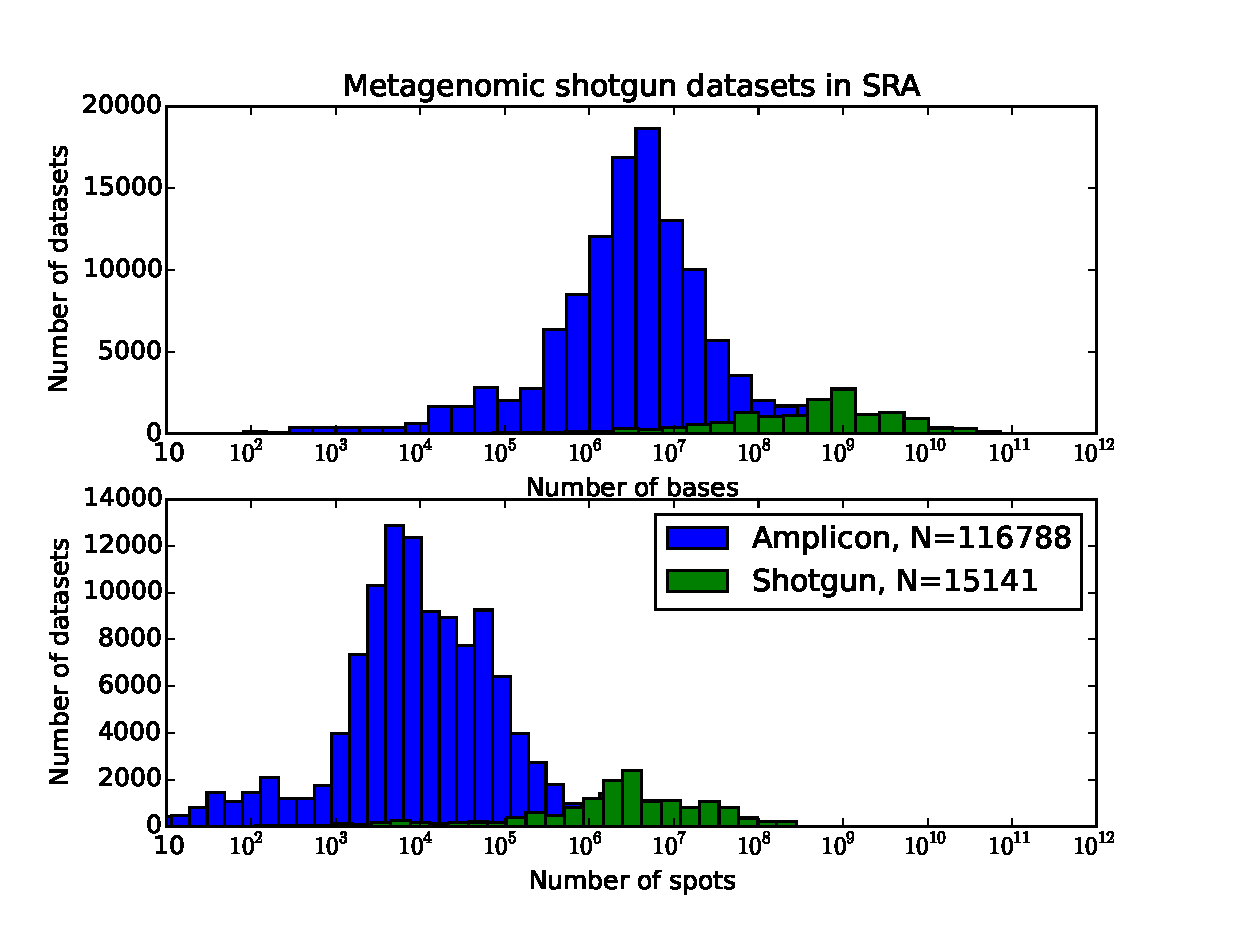
\includegraphics[width=11.5cm]{imgs/histogram.eps}
%
\label{fig:1}       % Give a unique label
\end{figure}

On the other side of the read-length continuum, some instruments produce very long ($>$3kbase) reads with very poor sequence quality--base call error rates above 10\% (Pacific Biosciences, Oxford Nanopore).   The anonymous nature of individual reads makes these poor choices for metagenomics unless complemented with Illumina data with high base accuracy.  The simultaneous inference of organism and corrected sequence is not currently feasible with only long-read low-quality data except perhaps in the lowest complexity samples. 


\begin{table}
\caption{Sequencing platforms suitable for metagenomic sequencing.}
\begin{tabular}{lrrrrrrrrrr}
Platform &  Read & Read & Raw   & Error &       &  Targeted & Shotgun  \\
      & length & number & yield &  rate &       &           &         \\
%Roche 454 &  400 & 200k &  & 3\% &  & OK &   \\
Iontorrent PGM 318 &  200,400 & 5M & 1-2 Gb / cell & 2\% &  & OK &   \\
Iontorrent Proton &  200 & 10M & 2 Gb / cell & 3\% &  & OK &   \\
Illumina Miseq &  2x100-2x300 & 16M & 3-5 Gb / cell & 1\% &  & * & * \\
Illumina Nextseq &  2x150 & 360M, 120M & 110 Gb / cell & 1\% &  & * & * \\
Illumina Hiseq & 2x100,2x150 & 160M*8 & 40 Gb / lane & 1\% &  & * & * \\
ABIsolid & 50 & 1.4G & 70G & 5\% &  &  &   \\
PacBio &  6000 & 50k &300M  & 15\% &  &  & Supplemental  \\
%PacBio CCS & 400 & 50k &  & <1\% &  &  &   \\
  \\
\end{tabular}
\end{table}


% Because of the high complexity of metagenomic samples, individual reads contribute little to the genetic characterization of the entire sample, and require recognition of some kind before they are invested with meaning.

\subsection{Library Types}
There are two main metagenomic library types/kits that we have tested thoroughly and can confidently recommend for metagenomic sequencing.  These are the TruSeq and the Nextera, both from Illumina, Inc.(San Diego, California). These two library types differ in their approach in two key components of metagenomic library generation: the fragmenting or shearing of the input material and the ligation of sequencing adapters and sample-identifying barcodes.  TruSeq libraries have been on the market longer, so there are more kits and biotechnology companies that cater to their creation. 
Nextera libraries are newer and, to date can only be made with Illumina reagent kits. 
% 
TruSeq library generation uses mechanical shearing in a sonicator to fragment the DNA and ligates adapters separately. 
Nextera library generation uses an engineered transposase enzyme to simultaneously fragment and ligate adapters to the input material. 
%
The TruSeq and Nextera approaches differ considerably in the amount of input material needed. TruSeq libraries require 500-1,000~ng of input DNA, while Nextera needs only 50~ng.  This makes Nextera libraries is particularly helpful with low biomass samples.
Because of the use of sonication instead of enzymatic incubation, TruSeq libraries give the user greater control over the insert size of library fragments.  

\subsection{Sample requirements }
\label{subsec:4}
%
% When creating metagenomic sequencing libraries the quality and quantity of the genetic material to be sequence is of great importance. 
Input DNA quantities for library preparation kits range from 1~ng to  1$\umu$g of material. It is important to make sure that the amount of genetic material available for library preparation falls within the range given by the kit's protocol.
%
Because library creation depends on creating fragments in size ranges that work well with the sequencing technology, and because fragments in the wrong size range can be filtered out during library creation,  the quality of the input nucleic acids has a large effect on library success. 
Even if a researcher has ample genetic material, if the material is not of good quality a robust library often cannot be made. 
Sample quality, referring to the survival of high-molecular-weight nucleic acids, depends on the circumstances of extraction and storage as well as properties of the sampling environment; samples taken from hot or acidic environments tend to have lower nucleic acid quality compared to samples from cold or more neutral environment.


\section{Wetlab protocol}

\subsection{Storage}
The proper storage of a sample also plays a role in overall sample quality.  Storage variables such as delay before storage, storage temperature, and storage time can drastically affect relative abundances of microorganisms.  Systematic studies have shown that samples stored at room temperature and at --4\degree\,C show loss of 16S diversity and storage-associated microbial composition biases\cite{Rubin2013Investigating}.  We recommend storing samples at --80\degree\,C as soon as possible after collection, avoiding free-thaw cycles, and consistent extraction following storage to reduce storage associated community shits.  

We have experience with the MoBio PowerSoil DNA isolation Kit.    

\subsection{Quantification}
DNA quantification is an essential step at many places in the library creation workflow because some of the steps in library preparation and sequencing are concentration-dependent.

For assessing the quantity of a sample after extraction we recommend Invitrogen’s Qubit Fluorometer. The Qubit utilizes a fluorescent dye that binds to nucleic acids to determine the starting concentrations.  We recommend avoiding the Nanodrop, as it consistently overestimates nucleic acid concentrations. Unlike the Nanodrop, the Qubit Fluorometer can discriminate between DNA and contaminants, such as RNA.
%
To assess the quality of the genetic material we recommend using Agilent’s 2100 Bioanalyzer or an agrose gel. Generally, high quality nucleic acids destined for metagenomic research will be free of any fragments below 100-200~bp.  If the number of fragments 200~bp outnumber the rest this is an indication of overfragmentation or low input quality.


\paragraph{Equipment}
\begin{svgraybox}
\begin{enumerate}
\item{    Invitrogen Qubit Fluorometer}
\item{      Covaris S-series system}
\item{      Wafergen’s Apollo 324 system}
\item{      Magnetic Stand or Rack (holds 1.5ml or 96 well plates)}
\item{      Thermocycler}
\item{      Sage Science’s Blue Pippin Prep}
\item{      Agilent 2100 Bioanalyer}
\end{enumerate}
\end{svgraybox}

\subsection{Positive and negative controls }

There are numerous controls utilized throughout metagenomic library preparation in order to ensure quality data. The first of these controls is the extraction blank, a negative control. When extracting DNA from metagenomic samples researchers should include 1-3 extraction blanks with the sample set. The researcher will then compare the quality and quantity of the extraction blank to the samples and if a sample is found to match the extraction blank it will be discarded as a false positive.
%
The second of these controls is the library blank and is used in the same manner as the extraction blank. Water will be run through the library preparation process in tandem with the samples and used to remove false positives from the set.
%
Use of a negative control during library preparation is more common during the PCR step and several negative controls will often be included. This is because primer-dimers will often be generated by PCR along with the amplified libraries. Researchers will use the nucleic acid concentration of the negative controls to determine the concentration of primer-dimers in any given sample, often called the background noise.
%
Researchers also employ positive controls in metagenomic preparation. These positive controls consist of sequences of DNA that are of high quality, well studied, and explicitly known. The most common positive control is called PhiX. These positive controls can either be spiked into the samples as an internal control or they can be run by themselves, separately barcoded, as an external control. The positive controls are then compared to the individual samples to help determine the quality of the library and the effectiveness of the library preparation method. 

\subsection{DNA Quantification}

We recommend starting with 500~ng of high-quality DNA for TruSeq metagenomic library prep, although lower quality and concentrations may be used. By contrast, the Nextera protocol is optimized for exactly 50~ng, and samples should be diluted to that level.

We recommend the following protocol:
\begin{enumerate}
\item{     Make a Qubit working solution by diluting the Qubit DNA reagent 1:200 in Qubit DNA buffer using a sterile plastic tube.}
\item{       Load 190~$\umu$\,L of Qubit working solution into tubes labeled standard 1 and 2.}
\item{       Add 10~$\umu$\,L of standard 1 solution and standard 2 solution to the appropriate tube and mix by vortexing for 2-3 seconds.}
\item{         Note: These are positive and negative controls used to calibrate the instrument.}
\item{       Load 198~$\umu$\,L of Qubit working solution into each individual assay tube.}
\item{       Add 2~$\umu$\,L of DNA to each assay tube and mix by vortexing 2-3 seconds. The final volume of this solution should equal 200~ul.}
\item{        Note: The amount of sample and working solution added to each assay tube can vary depending on concentration of the sample. The sample can vary between 1-20~ul, and the working solution can vary between 199-180~$\umu$\,L with the final volume equaling 200~ul. It is recommended to use 2~$\umu$\,L of sample to produce the most accurate results.}
\item{       Allow all the tubes to incubate at room temperature for 2 minutes.}
\item{       Select DNA assay on the Qubit Fluorometer. Select run a new calibration.}
\item{       Insert the tube containing Standard 1, close lid and press read.}
\item{       Remove standard 1 and repeat step 8 for standard 2.}
\item{      Insert sample, close lid and press read.}
\item{      Calculate concentration using dilution calculation on Qubit Fluorometer by selecting original volume of sample added to the assay tube.}
\item{      Repeat step 10 and 11 until all samples have been quantified.}
\end{enumerate}

\subsection{TruSeq Metagenomic Library Prep}
\subsubsection{ Insert Size Determination}

Insert size determination is an important consideration for all Illumina libraries.  Due to the enzymatic shearing of Nextera libraries, the ratio of DNA to enzyme and the enzymatic cut sites will determine the size distribution of a Nextera library.  For TruSeq library prep, however, the user has more control over the size distribution.  It is critically important to determine what library insert size will work best for your downstream analysis. Often, bioinformaticians will have a preference. We recommend consulting with the bioinformaticians that will be analyzing data before making your libraries. 

        The current generation of sequncing platforms produces reads with error rates that vary as a function of position in the read.  The deterioration of sequence quality results from imperfect extension reactions that cause the sequencing signal to fade in strength and contrast, in part due to contributions from non-synchronized populations of template molecules.  Paired-end sequencing, which initiates synthesis from primers on opposite ends of the sequencing template allows the high-quality bases to be drawn from both ends of the templates.  

Careful selection of the size of the template molecules further permits reads to overlap.  Libraries constructed so that the end of the first read overlaps with the end of the second are called "overlapping" libraries and allow the construction of longer composite reads, where the low-quality parts of each reads are complemented by redundant sequencing.  Read merging is computationally inexpensive compared to assembly.  When applied to well constructed libraries more than 90\% of paired reads can be found to overlap.  Variations in the overlap fraction between different samples likely result from differences in template length distribution, and to the extent that this affects annotation this may be one of the sources of library-construction biases that occur in annotation output as batch effects.
        
Getting 90\% overlap requires careful control of the insert size.  Templates that are too short result in more overlap (and less resulting sequence) than expected, reducing sequencing yield.  Templates that are too long result in non-overlapping sequences, or mixtures of non-overlapping and overlapping sequences.   When templates are much too short, shorter than the read length, the sequencer sequences the template and a piece of the normally unsequenced adapter on each end--resulting in reads that overlap for most of the beginning of the sequences, but that have unrelated artificial barcode sequences at their ends.   These sequences can be recovered bioinformatically, but are of lower value than optimally overlapping sequences.

\begin{figure}[t]
%\sidecaption[t]
\caption{Cartoons of possible insert sizes, with attention to overlap between paired reads.  The blue lines indicate DNA from the library and the red and orange lines indicate the forward and reverse adapters.}
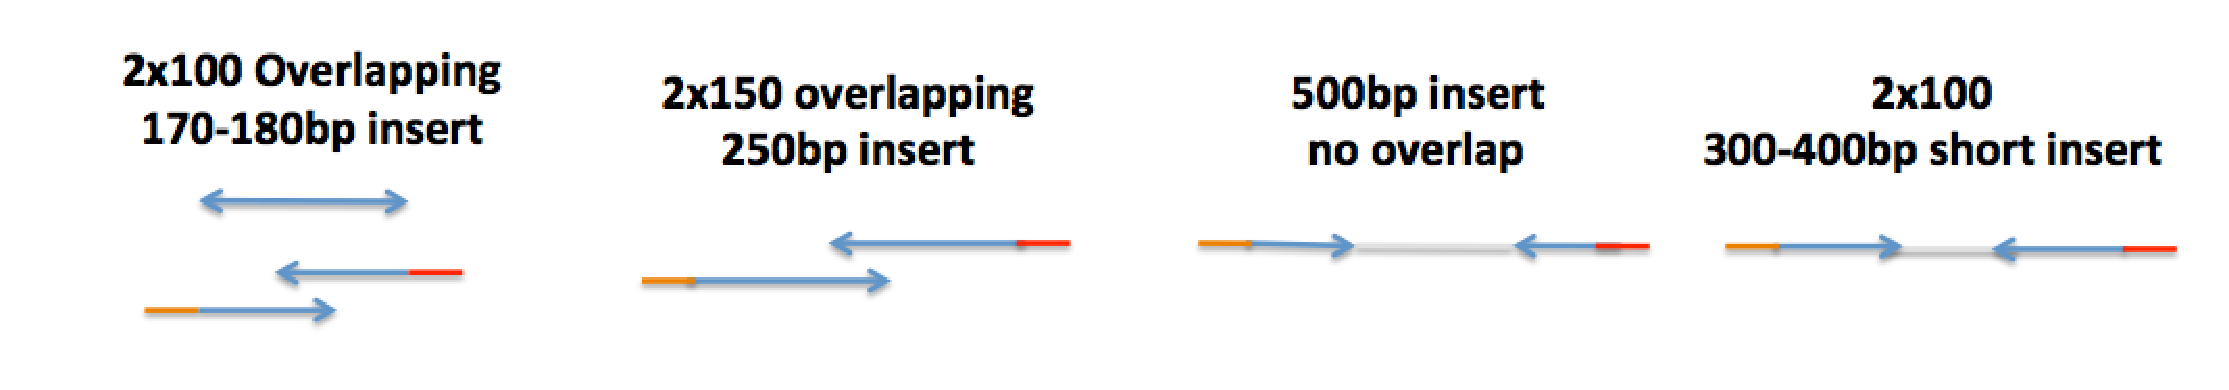
\includegraphics[width=11.5cm]{imgs/image1.eps}
%
\label{fig:1}       % Give a unique label
\end{figure}

For paired-end sequencing, insert sizes fall in several qualitatively different regimes, illustrated in Figure 1.    A 160-180 base pair insert (270-280~bp including adapters) will result in overlapping reads on a 2x100~bp Hiseq run, with 20-40~bp of overlap.  A 250 base pair insert  (350~bp with adapters) will result in overlapping reads on a 2x150 Hiseq run. A 500 base pair insert (600~bp with adapters) will result in no overlap on a 2X100 or 2X150 Hiseq run. Finally, a 350-450 base pair insert (450-550~bp with adapters) will result in no overlap with a known distance between the reads for single genome assembly.

\subsubsection{Shearing of Libraries}

For TruSeq libraries we recommend using the Covaris S-series system for mechanical shearing. The following instructions pertain to the S2 system but can be easily adapted to the S1 series.  We recommend setting the water bath between 6-8°C and using a minimum of 500~ng sample in 50~$\umu$\,L-100~$\umu$\,L. It is important to use no less than 50~$\umu$\,L of sample as the Covaris relies on surface area to appropriately shear the material.  If there is not at least 500~ng in 100~$\umu$\,L, we recommend using Agencourt Ampure XP Beads to concentrate the sample down to a smaller volume using a 1.8X bead ratio.  The conditions set on the Covaris are directly related to the preferred insert size of the final library, use the following table to determine what conditions to use for shearing.

\begin{table}
\label{shearingtable}
\caption{The input protocols for a S2 Covaris to achieve a peak at a given base pair length.}
\begin{tabular}{lrrrrrrrrrr}
Target Base Pair (Peak) & 150 & 200 & 300 & 400 & 500 & 800 & 1000 & 1500  \\
Duty Cycle & 10\% & 10\% & 10\% & 10\% & 5\% & 5\% & 5\% & 2\%  \\
Intensity & 5 & 5 & 4 & 4 & 3 & 3 & 3 & 4  \\
Cycles per Burst & 200 & 200 & 200 & 200 & 200 & 200 & 200 & 200  \\
Time (Seconds) & 430 & 180 & 80 & 55 & 80 & 50 & 40 & 15  \\
\end{tabular}
\end{table}

\subsubsection{Choosing barcodes and multiplexing}

When multiplexing, it is important to choose mixtures of barcodes that result in complementary color mixtures within 
the same pool/sequencing lane. Illumina Miseq and Hiseq instruments use four-color encoding, and 
bases A and C are principally found in the red channel while bases T and G are read out in the green channel. 
Mixtures of balanced color signals for each base--including the bases in the barcode--help the 
software maintain high data quality.
%During the index read, this 
%can be particularly challenging, as there are fewer bases present (just the indexes instead of the 
%biologically expected 25\% of each base). For example, if a pool only contained samples with index 
%1 and 2, during the first read of the index the machine would only detect samples in the red channel 
%(base A for index 1 and base C for index 2) and the quality of data would drop because the camera 
%would attempt to adjust focus due to the lack of samples in the green channel. 
We recommend choosing indexes for samples that allow for at least one base in each channel per pool.

\subsubsection{End repair, A-tailing, and Adapter Ligation on the Apollo 324}

After samples have been sheared, there are several different kits that will perform end-repair and ligation of A-tails and adapters. We recommend Illumina’s TruSeq PCR free Sample Prep, Illumina's Nano DNA Sample Prep Kits, Kapa Biosystems Library Amplification kits, or Wafergen’s PrepX Complete ILMN DNA library Kits. Each of these kits uses the same basic pipeline of end-repair, A-tail ligation, and adapter ligation and each will produce high quality libraries. The kits differ by the amount of input material they can handle, the insert size ranges they can produce, the time investment needed to complete the protocol, and the price. We prefer the Wafergen PrepX Complete ILMN DNA library kit as it has the fastest completion time and it is completed on an automated system allowing for less human error and increased reproducibility. It should be noted that the Kapa Biosystems Library Amplification kits can also be used on Wafergen’s Apollo 324 system. The following protocol pertains only to using Wafergen’s PrepX Complete ILMN DNA library Kits on Wafergen’s Apollo 324 system.

\subsubsection{PCR and Size Selection}

PCR and further size selection is not always necessary. For some applications the wide size distribution generated during library prep is sufficient. If the libraries are at least 2~nM concentration then PCR is unnecessary. If size selection is unnecessary start this protocol at step 9. If PCR is necessary we recommend using Bio-O Scientific’s NEXTflex DNA Barcodes and PCR mixture.  We recommend 10-15 cycles of PCR to achieve at least 2~nM concentration. If a tighter size distribution is necessary, we recommend further size selection with the Blue Pippin Prep (Sage Science, Inc., Beverly, MA), agarose gels, or E-Gels.  Each of these methods vary in the amount of input material they can handle, the insert size ranges they can produce, the time investment needed to complete the protocol, and the price. We prefer the Blue Pippin prep due to its ability to produce tighter sized libraries. The protocol below applies to the Blue Pippin Prep only. It is important to remember that we have accounted for the approximately 100~bp of adapter length to the library.  For instance, a 180~bp insert must be thought of as a 280~bp library. Thus we will size select for 100~bp larger than the given insert size to accommodate for the adapters.
We recommend the following protocol:
\begin{enumerate}
\item{1.      Choose the appropriate cassette to the given insert size and library size}
\item{a.      3\% cassette ranges from 90-200~bp}
\item{b.      2\% cassette ranges from 100-600~bp}
\item{c.      1.5\% cassette ranges from 250~bp-1.5kb}
\item{d.      0.75\% cassette ranges from 1-50kb}
\item{2.      Program the Pippin}
\item{a.      In the Blue Pippin software go to the Protocol Editor tab}
\item{b.      Click on the Cassette folder that matches the appropriate cassette for the given library size}
\item{c.      Select either “range” or “tight” and enter in the given base pair range or peak}
\item{d.      Click the “use internal standards” button}
\item{3.      Calibrate the Optics}
\item{a.      Place the calibration fixture in the optical nest, close the lid and hit “calibrate.”}
\item{b.      Continue only if it passes, if it does not pass, try again.}
\item{4.      Load the Cassette}
\item{a.      Inspect the cassette from bubbles, breakage of agarose column, and equal buffer levels.}
\item{b.      Dislodge any bubbles from the elution chamber}
\item{c.      Place the cassette into the optics nest}
\item{d.      Fill the sample well to the top with buffer}
\item{e.      Remove any buffer from the elution well and fill it with 40~$\umu$\,L of fresh buffer.}
\item{f.      Place a seal over the elution wells to keep them from overflowing during the run}
\item{g.      Run a continuity test and continue only if it passes. Try again if it fails.}
\item{5.      Mix the library and dye}
\item{a.      Mix at least 30~$\umu$\,L of library with 10~$\umu$\,L of dye. If there is less then 30~$\umu$\,L use nuclease-free water to dilute the libraries to 30~ul.}
\item{b.      Vortex the libraries and dye well and spin the mixture down}
\item{6.      Load the samples}
\item{a.      Remove 40~$\umu$\,L of buffer from the sample well and replace it with the 40~$\umu$\,L mixture of sample and dye.}
\item{b.      Repeat for each sample}
\item{c.      Close the lid and hit the “start” button}
\item{7.      The Blue Pippin will run for 30-56 minutes depending on the given program}
\item{8.      Open the lid, remove the samples from the elution wells and place into a collection tube}
\item{9.      Check the concentration of the samples with a DNA HS assay on the Qubit Fluorometer as referenced above}
\item{10.      Use the Qubit concentration and estimated library size (100~bp + insert size) to calculate the molarity of the sample with the following equation (with X= ng/$\umu$\,L concentration and Y= estimated size of fragment in bp): Molarity in nM = [X/1*10-6]/[Y*660]}
\item{11.     If the estimated molarity is less the 2~nM then proceed to PCR in step 12. If it is 2~nM or higher proceed to final library quantification}
\item{12.     PCR using Bio-O Scientific’s NEXTflex\textsuperscript{TM} DNA Barcodes and PCR mixture}
\item{a.      Mix 7.5~$\umu$\,L of the library, 29.5~$\umu$\,L of nuclease-free water, 12~$\umu$\,L of NEXTflex\textsuperscript{TM} PCR master mix, and 2~$\umu$\,L NEXTflex\textsuperscript{TM} Primer Mix in a well of a PCR strip tube or plate.}
\item{b.      Set a pipette to 50~$\umu$\,L and mix by pipetting up and down 10 times}
\item{c.      PCR on a thermocycler under the following settings}
\item{i.      2 minutes at 98°C}
\item{ii.     10-15 cycles of: 30 seconds at 98°C, 30 seconds at 65°C, 60 seconds at 72°C}
\item{iii.    4 minutes at 72°C}
\item{d.      Add 44~$\umu$\,L of AMPure XP Beads}
\item{e.      Incubate at room temperature for 15 minutes. During incubation, prepare an 80\% ethanol solution.}
\item{f.      Place the tubes or plate on the magnetic stand at room temperature for at least 5 minutes, until the liquid appears clear.}
\item{g.      Remove and discard the supernatant from each tube. Do not disturb the beads.}
\item{h.      With the samples still on the magnetic stand, add 200~$\umu$\,L of freshly prepared 80\% ethanol to each sample, without disturbing the beads.}
\item{i.      Incubate at room temperature for at least 30 seconds while still on the magnetic stand, then remove and discard all of the supernatant from each tube. Again, do not disturb the beads.}
\item{j.      Repeat steps 6 and 7 one more time for a total of two 80\% ethanol washes.}
\item{k.      Allow the tubes to air dry on the magnetic stand at room temperature for 15 minutes or until the beads no longer appear wet.}
\item{l.      Add 15~$\umu$\,L of nuclease-free water to each tube.}
\item{m.      Thoroughly resuspend the beads by gently pipetting 10 times.}
\item{n.      Incubate the tubes at room temperature for 2 minutes.}
\item{o.      Place the tubes back onto the magnetic stand at room temperature for at least 5 minutes, until the liquid appears clear.}
\item{p.      Transfer the clear supernatant from each tube to an appropriate collection tube. Leave at least 1~$\umu$\,L of the supernatant behind to avoid carryover of magnetic beads.}
\item{13.     Proceed to Final Library Quantification}
\end{enumerate}

\subsection{Nextera Metagenomic Library Prep}

For metagenomic library prep of low biomass samples, we recommend using Illumina’s Nextera DNA kit. It is important that exactly 50~ng of sample is used as this protocol is optimized for exactly 50~ng. The sample should be in a 20~$\umu$\,L volume at a concentration of 2.5~ng/ul. If the sample has 50~ng but is in a volume that is larger than 20~ul, a 1.8X ratio of Agencourt Ampure XP Beads can be used to bring the sample to the appropriate volume.  Please note that all of the abbreviations in this protocol refer to abbreviations used to describe reagents in the Illumina Nextera DNA kit.

\subsubsection{Tagmentation of Genomic DNA}

In this step the transposome fragments the DNA while adding adapter sequences to the ends, allowing it to be amplified by PCR in later steps; our protocol includes a 5 minute incubation at 55\degree\,C.

\subsubsection{Clean-up of Tagmented DNA}

This step is critical because without it the Nextera transposome can bind tightly to the DNA and will interfere with downstream processing.  We recommend using ZymoTM Purification Kit (ZR-96 D NA clean and Concentrator TM-5) for this protocol. 

\subsubsection{Choice of barcodes }

% Barcodes are packaged in kits; we prefer Illumina's barcodes.  
Nextera libraries are dual-indexed, meaning that each sample has two barcodes (an i7 and i5 index) ligated on opposite adapter/primers.  It is important to ensure that no two samples in the same pool have the exact same combination of indexes. We recommend arranging samples in a 96 well plate and to assign each column an i7 index and each row an i5 index when working with moderate numbers of samples. 

When multiplexing, it is also important to choose barcodes for individual samples that will be color-complementary with the barcodes of other samples in a given pool, avoiding mixtures of barcodes with extreme signals in the green and red channels.
Illumina Miseq and Hiseq instruments use four-color encoding, and bases A and C are principally found in the red channel while bases T and G are read out in the green channel.
 For example, if only samples with index 701(TAAGGCGA) and 704(TCCTGAGC) were in a pool, during the first read of the index the machine would only detect samples in the green channel (base T for index 1 and base T for index 2).  This deprives the machine of the color contrast that it requires to identify clusters and issue confident base calls.  We recommend choosing indexes for samples that allow for at least one base in each channel per pool. For Nextera libraries it is also important to achieve red-green channel balance for both the i7 and i5 index mixtures separately. 

\subsubsection{PCR Amplification}
It is critical to use the full amount of recommended input DNA at this step to ensure libraries that produce high quality sequencing results. 

\subsection{Final Library Quantification}

The molarity and library size are critical for successful clustering and sequencing.  Figure 2 shows examples of Bioanalayzer scans of completed library types. Illumina recommends that completed libraries achieve a molarity of at least 2~nM or greater in order to be sequenced with quality results.  It is important to remove any primer-dimers that may be present. Primer-dimers will be visible on a Bioanalyzer electropherogram between bases 0-100 depending on the length of PCR primers you are using. If primer-dimers are present use a 1X ratio of AMPure XP Beads to remove them. To assess the quality of the completed library, we recommend the following protocol:
\begin{enumerate}
\item{      Use the Qubit Fluorometer to determine the concentration of libraries in ng/ul, as referenced above.}
\item{      Use the Agilent 2100 Bioanalyzer to determine the library insert size and length. As referenced above.}
\item{      Use the concentration from the Qubit and peak base pair size generated by the Bioanalyzer to calculate the molarity of the sample with the equation provided above.}
\item{      The libraries are considered complete and ready for Illumina sequencing if the molarity is 2~nM or greater.}
\end{enumerate}

\begin{figure}
%\sidecaption[t]
\caption{Bioanalyzer traces of complete libraries. Panel a shows a TruSeq library with a narrow range peaking around 1kb. Panel b shows a a TruSeq library with a narrow range peaking around 360~bp. Panel c shows a TruSeq library with a narrow range peaking around 700~bp. Panel d shows a TruSeq library with a broad range peaking around 450~bp. Panel e shows a Nextera library peaking around 1,600~bp.  }
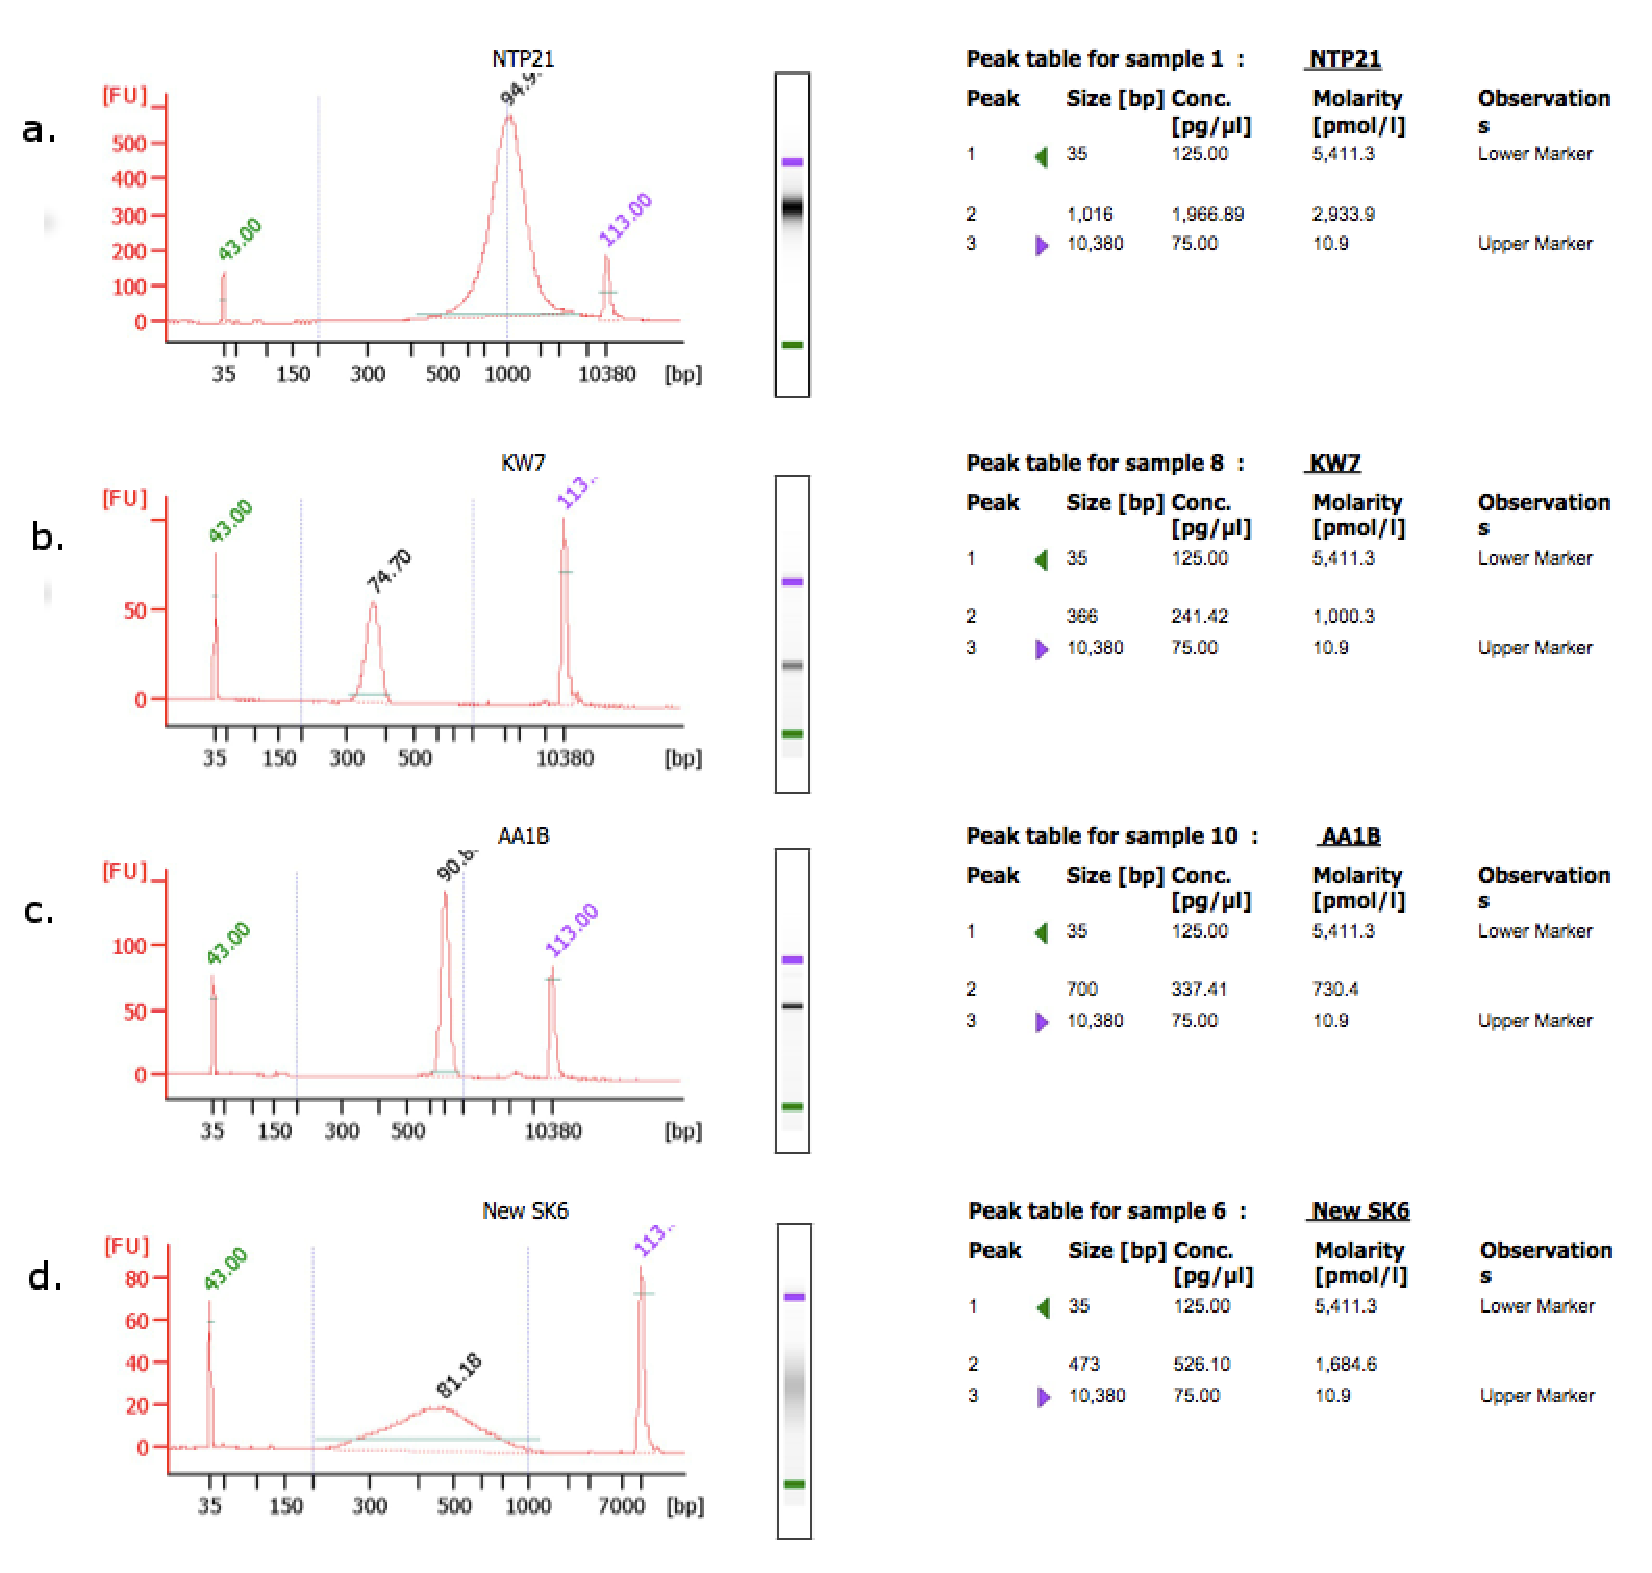
\includegraphics[width=12cm]{imgs/ABCD.eps}
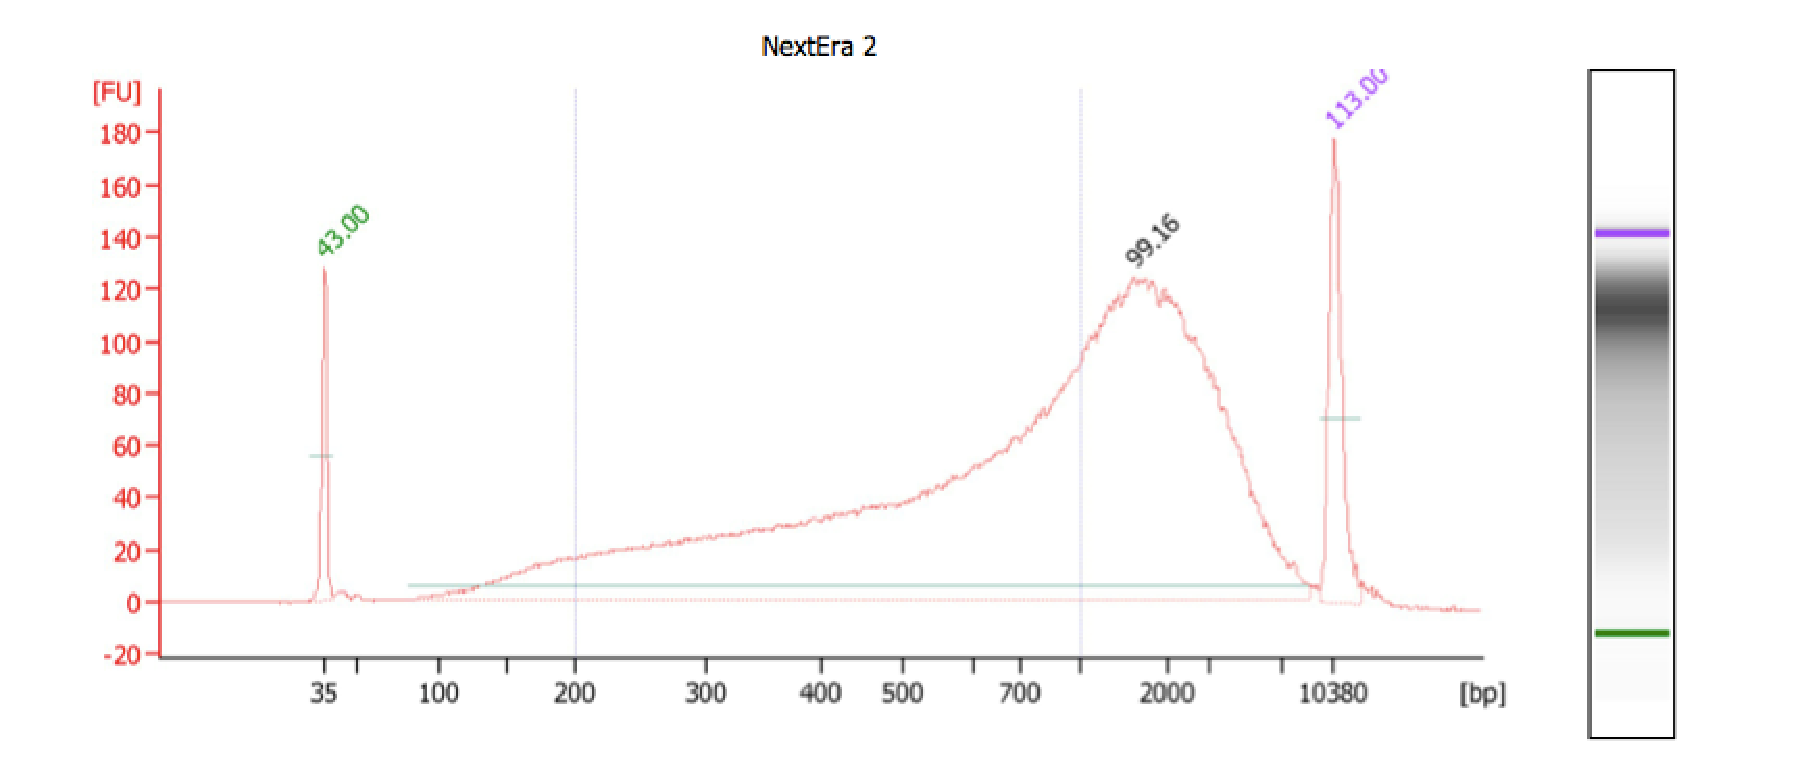
\includegraphics[width=6cm]{imgs/image6.eps}
%
%\caption{Please write your figure caption here}
% \caption{ }
% If the width of the figure is less than 7.8 cm use the \texttt{sidecapion} command to flush the caption on the left side of the page. If the figure is positioned at the top of the page, align the sidecaption with the top of the figure -- to achieve this you simply need to use the optional argument \texttt{[t]} with the \texttt{sidecaption} command}
\label{fig:2}       % Give a unique label
\end{figure}

\section{Analysis}
\label{sec:4}

\subsection{Sequence complexity}
Nucleic acid sequences determined from environmental samples are difficult to interpret for a variety of reasons, and as a result exploitation of metagenomic shotgun data is computationally expensive compared to the study of model organisms.
Some parts of microbial genomes evolve quickly and make detection of similarity technically difficult.
Many environmental microbes and microbial genes lack close relatives in cultured organisms, resulting in large fractions of many environmental samples going unannotated.
Environmental samples present a formidable inference problem of unraveling unknown mixtures of anonymous organisms.  When this problem has been approached, expectation-maximization has been the algorithmic workhorse.
Unlike the sequencing of reference organisms, where the complexity of the sequence is limited by the genome of the underlying organism, environmental samples sometimes show diversity whose limits have not yet been circumscribed by observations.  This exceedingly high observed sequence diversity makes some datasets fail to compress, and exposes the annotation procedure to gigabases of raw data for annotation.

High-throughput sequencing datasets of typical size ($10^{8}--10^{11}~$bp) are too large for routine handling by general-purpose desktop and laptop computers.  These datasets are also too large for BLAST--faster, presumably less sensitive algorithms are the only choice for tens of millions of reads at a time; BLAST is affordable only for value-added sequences, not raw short-read data.

\subsection{Open and closed}
The analysis of both targeted-gene and shotgun sequencing can proceed according to two general approaches, depending on whether inferences about the sequence content of the samples depend on the databases used for comparison and interpretation.  These approaches are called closed-reference and open-reference.  Open-reference approaches are presumably more powerful, but involve unknown sample-dependent biases that cause the completeness of the analytical representation of the sequences to vary.

Comparing new sequence data to a database of sequences or sequence signatures is called "closed-reference annotation."  Closed-reference annotation has the advantages that datasets annotated using the same procedure can be reliably compared because the space of possible annotations is limited and can be known in advance.
Experience has shown that DNA recruitment of environmental samples to the genomes of all cultivated organisms often explains low (10-50\%) fractions of the dataset, leaving 50-90\% of environmental shotgun sequences without recognizable similarity to database sequences.

% (XXXX PIPELINE REVIEW, or at least pipeline list)  (MG-RAST, HUMANN, MEGAN, imicrobe, IMG/M, CAMERA... )

Constructing sequence hypotheses from the data and performing a database-comparison annotation on value-added sequences is called open reference annotation.   For targeted gene sequencing, the sequence hypotheses are clusters constructed from the observed data; for shotgun sequencing, hypotheses are usually the products of sequence assembly of the shotgun data.   Unlike closed-reference annotation, open-reference annotation can discover and describe sequence patterns present in the data but not in the database.  Open-reference annotation is more technically tricky and suffers from uncharacterized biases in the sequence construction phase, and difficulty in interpretation of the results.  The sequences resulting from assembly, called contigs, are longer and can contain both complete genes and chains of genes from the same organism, permitting better resolution when comparing to databases and allowing analysis of synteny in metagenomic data.

The increased value of the sequences in open-reference annotation, however, comes with added analytical complexity.   
The collection of all the assembled contigs is always an incomplete summary of the metagenomic dataset, and contigs are not of equal importance in light of the sequence data.
Contigs vary both in length and in depth, and the effects of this heterogeneity, which depends on uncontrolled properties of the sample and its biological diversity, on analysis are as yet unexplored.

The growing nature of the set of reference sequences in open-reference (assembly-based) analysis of shotgun metagenomic data means that sequences are typically analyzed in batches using defined sets of reference sequences, and comparisons of sample sets between lots with different sets of references are not straightforward.

\subsection{Analysis Workflow overview}
        To address artifacts associated with sequencing technology and to improve ultimate signal-to-noise, metagenomic data are subjected to a number of sequence-level filters before assembly or annotation.  These preprocessing steps remove uninformative sequences, correct low-level errors, and discard sequence subsets enriched in errors.

        Removal of known sequence contaminants or positive control spikes is computationally straightforward when the contaminating sequences are known.   Samples of host-associated microbes may contain varying amounts of host DNA, and the varying host content of the samples (or perhaps other host characteristics) represent an unwanted, potentially confounding signal in the genetic analysis of microbial community composition.  Reads are compared to the reference genome with a fast read aligner (bwa and bowtie2 are the current state of the art) and reads that match are excluded from further analysis.   Fecal samples from humans and animals, samples of wounds, and plant-associated sampling are all subject to this sort of confounding from host-organism contamination. 

        Current sequencing technologies each have platform-specific artificial sequences which are part of the sequencing technology.  These include PCR primers,  barcodes, and linker sequences that are ligated onto the sequences of interest.
For some protocols, these sequences are intended to appear in the output, but in the standard Illumina single-end and paired-end protocols, adapter sequences in the sequence output are a symptom of poorly-executed sequencing library preparation, either bad sequence size selection or survival of primer-dimers to the sequencing stage.
These contaminants can include as few as 30~bp and as much as 150~bp of distinct sequence.   Removing these "adapter" sequences is not computationally expensive, but there are no generally accepted guidelines on how much contamination is acceptable.  Contamination ranges from minimal, affecting less than $10^{-5}$ of reads in a dataset, to as much as half of some sequence datasets; $10^{-3}$ is typical. 
Adapter sequences are a bigger problem for assembly than for recruitment or annotation.

\subsection{The human factor}
Just as with laboratory technicians, bioinformatic data processing requires people with specialized skills.  The bioinformatic handling of any sort of sequencing data requires computational competency, including familiarity with transport, storage, and format conversion of large data files; management of maintainable workflows; ability to navigate sequence archives for sets of relevant reference sequences; and the ability to replicate computational workflows described in the literature, which requires installing and troubleshooting software.

Researchers usually get better results by sharing research goals, hypotheses, and prior information with the specialists, both in the wetlab and on the computational end.  In order to suggest or apply procedures in the wetlab or in the computer lab to attenuate unwanted, contaminating DNA or sequences technicians need to know what signals are interesting, and what likely uninformative signals look like.  These specialists cannot help you if you give them DNA and sample numbers and no further instructions.  

\section{Reporting }
\label{sec:5}

The output from an Illumina Next Generation sequencing run is ultimately one or more FASTQ files.\cite{Cock2010FASTQ} 
Metagenomes will be analyzed using the available online resources (e.g. IMG/M, MGRAST, CAMERA, EBIs Metagenomics portal, etc.) providing annotation by comparing transcripts to different functional gene databases (e.g. using BLAST to assign functions against M5NR, SFams and SEED). For more detailed descriptions of potential functional pipelines and analyses of these data see \cite{Thomas2012Metagenomics}, \cite{Meyer2008Metagenomics} \cite{Wilke2015RESTful}

        The results of closed-reference annotation are per-sample "feature vectors" representing the number of observations of biological molecules of a given type.  The number of dimensions of this vector can range from a handful (classifying reads merely by estimated domain) to millions (counting each database sequence as a distinct potential unit of observation), and in general the number of observable features far exceeds the number of samples.

        Raw shotgun metagenomics datasets range from hundreds of megabytes to hundreds of gigabytes in size.  Since 2009 the NCBI's Sequence Read Archive has archived raw data from sequencing runs with mandatory metadata on protocol, sampling, and sequencing.  The archive issues accession numbers for individual samples, individual instrument runs, collections of runs with the same protocol, collections of runs with the same purpose but different protocols, and collections of sequencing experiments with different samples, and has some features for accessioning analysis products.  
In addition to the public archives, some annotation services (MG-RAST, iMicrobe, and IMG/M) host metagenomic sequence data and annotation results and allow making public raw and value-added sequence data.    NCBI's Whole Genome Shotgun archive accepts assembled contigs in FASTA format if sufficient metadata are provided, and is one option for making contigs available for later use for comparative study.
Some consortia have published their value-added data products (for example annotation tables, results from assemblies) separately from the public sequence archives.

The accession numbers from depositions of the raw read data and of assemblies derived from the data must be included and associated with sample names when publishing results using metagenomic sequencing.  

\section{Government license}

The submitted manuscript has been created by UChicago Argonne, LLC, Operator of Argonne National Laboratory ("Argonne").  Argonne, a U.S. Department of Energy Office of Science laboratory, is operated under Contract No. DE-AC02-06CH11357.  The U.S. Government retains for itself, and others acting on its behalf, a paid-up nonexclusive, irrevocable worldwide license in said article to reproduce, prepare derivative works, distribute copies to the public, and perform publicly, and display publicly, by or on behalf of the Government.

%\label{sec:6}

% For figures use
%

% Use the \index{} command to code your index words

%
% \begin{acknowledgement}
%If you want to include acknowledgments of assistance and the like at the end of an individual chapter please use the \verb|acknowledgement| environment -- it will automatically render Springer's preferred layout.
% \end{acknowledgement}
%

% %%%%%%%%%%%%%%%%%%%%%%%% referenc.tex %%%%%%%%%%%%%%%%%%%%%%%%%%%%%%
% sample references
% %
% Use this file as a template for your own input.
%
%%%%%%%%%%%%%%%%%%%%%%%% Springer-Verlag %%%%%%%%%%%%%%%%%%%%%%%%%%
%
% BibTeX users please use
% \bibliographystyle{}
% \bibliography{}
%
\biblstarthook{References may be \textit{cited} in the text either by number (preferred) or by author/year.\footnote{Make sure that all references from the list are cited in the text. Those not cited should be moved to a separate \textit{Further Reading} section or chapter.} The reference list should ideally be \textit{sorted} in alphabetical order -- even if reference numbers are used for the their citation in the text. If there are several works by the same author, the following order should be used: 
\begin{enumerate}
\item all works by the author alone, ordered chronologically by year of publication
\item all works by the author with a coauthor, ordered alphabetically by coauthor
\item all works by the author with several coauthors, ordered chronologically by year of publication.
\end{enumerate}
The \textit{styling} of references\footnote{Always use the standard abbreviation of a journal's name according to the ISSN \textit{List of Title Word Abbreviations}, see \url{http://www.issn.org/en/node/344}} depends on the subject of your book:
\begin{itemize}
\item The \textit{two} recommended styles for references in books on \textit{mathematical, physical, statistical and computer sciences} are depicted in ~\cite{science-contrib, science-online, science-mono, science-journal, science-DOI} and ~\cite{phys-online, phys-mono, phys-journal, phys-DOI, phys-contrib}.
\item Examples of the most commonly used reference style in books on \textit{Psychology, Social Sciences} are~\cite{psysoc-mono, psysoc-online,psysoc-journal, psysoc-contrib, psysoc-DOI}.
\item Examples for references in books on \textit{Humanities, Linguistics, Philosophy} are~\cite{humlinphil-journal, humlinphil-contrib, humlinphil-mono, humlinphil-online, humlinphil-DOI}.
\item Examples of the basic Springer style used in publications on a wide range of subjects such as \textit{Computer Science, Economics, Engineering, Geosciences, Life Sciences, Medicine, Biomedicine} are ~\cite{basic-contrib, basic-online, basic-journal, basic-DOI, basic-mono}. 
\end{itemize}
}

\begin{thebibliography}{99.}%
% and use \bibitem to create references.
%
% Use the following syntax and markup for your references if 
% the subject of your book is from the field 
% "Mathematics, Physics, Statistics, Computer Science"
%
% Contribution 
\bibitem{science-contrib} Broy, M.: Software engineering --- from auxiliary to key technologies. In: Broy, M., Dener, E. (eds.) Software Pioneers, pp. 10-13. Springer, Heidelberg (2002)
%
% Online Document
\bibitem{science-online} Dod, J.: Effective substances. In: The Dictionary of Substances and Their Effects. Royal Society of Chemistry (1999) Available via DIALOG. \\
\url{http://www.rsc.org/dose/title of subordinate document. Cited 15 Jan 1999}
%
% Monograph
\bibitem{science-mono} Geddes, K.O., Czapor, S.R., Labahn, G.: Algorithms for Computer Algebra. Kluwer, Boston (1992) 
%
% Journal article
\bibitem{science-journal} Hamburger, C.: Quasimonotonicity, regularity and duality for nonlinear systems of partial differential equations. Ann. Mat. Pura. Appl. \textbf{169}, 321--354 (1995)
%
% Journal article by DOI
\bibitem{science-DOI} Slifka, M.K., Whitton, J.L.: Clinical implications of dysregulated cytokine production. J. Mol. Med. (2000) doi: 10.1007/s001090000086 
%
\bigskip

% Use the following (APS) syntax and markup for your references if 
% the subject of your book is from the field 
% "Mathematics, Physics, Statistics, Computer Science"
%
% Online Document
\bibitem{phys-online} J. Dod, in \textit{The Dictionary of Substances and Their Effects}, Royal Society of Chemistry. (Available via DIALOG, 1999), 
\url{http://www.rsc.org/dose/title of subordinate document. Cited 15 Jan 1999}
%
% Monograph
\bibitem{phys-mono} H. Ibach, H. L\"uth, \textit{Solid-State Physics}, 2nd edn. (Springer, New York, 1996), pp. 45-56 
%
% Journal article
\bibitem{phys-journal} S. Preuss, A. Demchuk Jr., M. Stuke, Appl. Phys. A \textbf{61}
%
% Journal article by DOI
\bibitem{phys-DOI} M.K. Slifka, J.L. Whitton, J. Mol. Med., doi: 10.1007/s001090000086
%
% Contribution 
\bibitem{phys-contrib} S.E. Smith, in \textit{Neuromuscular Junction}, ed. by E. Zaimis. Handbook of Experimental Pharmacology, vol 42 (Springer, Heidelberg, 1976), p. 593
%
\bigskip
%
% Use the following syntax and markup for your references if 
% the subject of your book is from the field 
% "Psychology, Social Sciences"
%
%
% Monograph
\bibitem{psysoc-mono} Calfee, R.~C., \& Valencia, R.~R. (1991). \textit{APA guide to preparing manuscripts for journal publication.} Washington, DC: American Psychological Association.
%
% Online Document
\bibitem{psysoc-online} Dod, J. (1999). Effective substances. In: The dictionary of substances and their effects. Royal Society of Chemistry. Available via DIALOG. \\
\url{http://www.rsc.org/dose/Effective substances.} Cited 15 Jan 1999.
%
% Journal article
\bibitem{psysoc-journal} Harris, M., Karper, E., Stacks, G., Hoffman, D., DeNiro, R., Cruz, P., et al. (2001). Writing labs and the Hollywood connection. \textit{J Film} Writing, 44(3), 213--245.
%
% Contribution 
\bibitem{psysoc-contrib} O'Neil, J.~M., \& Egan, J. (1992). Men's and women's gender role journeys: Metaphor for healing, transition, and transformation. In B.~R. Wainrig (Ed.), \textit{Gender issues across the life cycle} (pp. 107--123). New York: Springer.
%
% Journal article by DOI
\bibitem{psysoc-DOI}Kreger, M., Brindis, C.D., Manuel, D.M., Sassoubre, L. (2007). Lessons learned in systems change initiatives: benchmarks and indicators. \textit{American Journal of Community Psychology}, doi: 10.1007/s10464-007-9108-14.
%
%
% Use the following syntax and markup for your references if 
% the subject of your book is from the field 
% "Humanities, Linguistics, Philosophy"
%
\bigskip
%
% Journal article
\bibitem{humlinphil-journal} Alber John, Daniel C. O'Connell, and Sabine Kowal. 2002. Personal perspective in TV interviews. \textit{Pragmatics} 12:257--271
%
% Contribution 
\bibitem{humlinphil-contrib} Cameron, Deborah. 1997. Theoretical debates in feminist linguistics: Questions of sex and gender. In \textit{Gender and discourse}, ed. Ruth Wodak, 99--119. London: Sage Publications.
%
% Monograph
\bibitem{humlinphil-mono} Cameron, Deborah. 1985. \textit{Feminism and linguistic theory.} New York: St. Martin's Press.
%
% Online Document
\bibitem{humlinphil-online} Dod, Jake. 1999. Effective substances. In: The dictionary of substances and their effects. Royal Society of Chemistry. Available via DIALOG. \\
http://www.rsc.org/dose/title of subordinate document. Cited 15 Jan 1999
%
% Journal article by DOI
\bibitem{humlinphil-DOI} Suleiman, Camelia, Daniel C. O�Connell, and Sabine Kowal. 2002. `If you and I, if we, in this later day, lose that sacred fire...�': Perspective in political interviews. \textit{Journal of Psycholinguistic Research}. doi: 10.1023/A:1015592129296.
%
%
%
\bigskip
%
%
% Use the following syntax and markup for your references if 
% the subject of your book is from the field 
% "Computer Science, Economics, Engineering, Geosciences, Life Sciences"
%
%
% Contribution 
\bibitem{basic-contrib} Brown B, Aaron M (2001) The politics of nature. In: Smith J (ed) The rise of modern genomics, 3rd edn. Wiley, New York 
%
% Online Document
\bibitem{basic-online} Dod J (1999) Effective Substances. In: The dictionary of substances and their effects. Royal Society of Chemistry. Available via DIALOG. \\
\url{http://www.rsc.org/dose/title of subordinate document. Cited 15 Jan 1999}
%
% Journal article by DOI
\bibitem{basic-DOI} Slifka MK, Whitton JL (2000) Clinical implications of dysregulated cytokine production. J Mol Med, doi: 10.1007/s001090000086
%
% Journal article
\bibitem{basic-journal} Smith J, Jones M Jr, Houghton L et al (1999) Future of health insurance. N Engl J Med 965:325--329
%
% Monograph
\bibitem{basic-mono} South J, Blass B (2001) The future of modern genomics. Blackwell, London 
%
\end{thebibliography}

\bibliographystyle{plain}
\bibliography{metagenomics.bib}

\end{document}
